\section{Algorithmic Background}
\label{section:background}
\par
{\bf SPOOLES} is an attempt to provide the capability for solving
sparse systems of linear equations for a diverse set of applications 
on a diverse set of parallel computers.  We have included innovative
approaches for the ordering of sparse matrices.  We have also taken
an object oriented approach to providing the sparse matrix technology
which is different from the more traditional subroutine library
approach.  The algorithms for the numerical factorization and
solve steps are based on established algorithms.
\par
The purpose of this chapter is to give a quick overview of the
algorithms used in {\bf SPOOLES}.  We will leave the complete
description of the algorithms to the references.
\par
\subsection{Ordering a sparse matrix}
\label{subsection:intro:ordering}
\par
The past few years have seen a resurgence of interest and
accompanying improvement in algorithms and software to order sparse
matrices.
The minimum degree algorithm, specifically the multiple external
minimum degree algorithm \cite{liu85-mmd},
was the preferred algorithm of choice for
the better part of a decade.
Alternative minimum priority codes have recently pushed multiple
minimum degree aside,
including approximate minimum degree \cite{ame96-amd} and
approximate deficiency \cite{ng96-mindefIdaho},
\cite{rot96-mindefIdaho}.
They offer improved quality or improved run time, and on occasion,
both. 
\par
Nested dissection for regular grids \cite{geo73-nested} is within a
factor of optimal with respect to factor entries and operation counts.
One of the earliest attempts, automatic nested dissection 
\cite{geo81-book} used a simple profile algorithm to find separators.
It rarely performed as well as minimum degree.
Better heuristics to find separators were brought in from the
electrical device simulation area \cite{lei89-fidmat} and while
these algorithms produced better orderings, the run times kept
them from practical application.
Nested dissection came on its own with two developments.
The first was the application of spectral analysis of graphs to
find separators \cite{pot90-partition}.
The eigenvector associated with the smallest nonzero eigenvalue of
the Laplacian of a graph generates a spectrum of separators.
While the ordering times for spectral nested dissection were still
on the order of ten or more times the cost of a minimum degree ordering,
the ordering quality sometimes made the cost worthwhile.
\par
The key that made nested dissection a competitive and practical
alternative to minimum degree was the introduction of multilevel
ideas ---
to find a separator on a graph, first find a separator on a coarse
graph and project back to the original.
Early implementations include \cite{bar93-partition}
and \cite{bui93-partition}.
Multilevel algorithms are very popular in current software
including
{\bf CHACO}
\cite{hen93-chaco},
\cite{hen93-partition},
{\bf METIS}
\cite{kar95-multilevel},
\cite{kar95-metis},
{\bf BEND}
\cite{hr96-msnd},
{\bf WGGP}
\cite{gup96-WGPP}
and
{\bf PCO}
\cite{rag95-PCO}.
\par
{\bf SPOOLES} also includes a hybrid ordering approach called
multi-section 
\cite{ash95-DDSEP},
\cite{ash96-maxflow},
\cite{ash96-multisection} and
\cite{ro95-hybrid}.
For some types of graphs, nested dissection does much better than
minimum degree, for others much worse.
Multisection is an ordering that uses both nested dissection and
minimum degree to create an ordering that is almost always as good
or better than the better of nested dissection or minimum degree
and rarely much worse.
\par
\subsection{Background on permutations and trees}
\label{subsection:order:background}
\par
Two important structures that are used in the solution of sparse
systems of equations are permutations and trees.  Because of the
object oriented nature of the {\bf SPOOLES} library the user
needs to know some information about these structures.
\par
For an example, let us examine the matrix R2D100, a matrix generated by
first randomly triangulating the unit square with 100 grid points.
The resulting matrix has 100 rows and columns.
We ordered the matrix using a generalized nested dissection
algorithm from the {\bf SPOOLES} library, and present the
vertex elimination tree for this ordering in
Figure~\ref{fig:R2D100-tree-vtx}.  The vertex elimination tree is
a representation of the order that the vertices in the graph
will be eliminated.  
This order corresponds to the order that the rows
and columns will be factored for a square $A$.
The dependencies of the order form a tree structure.  
The leaves of the tree (our trees hang 
upside down with the leaves at the bottom and the root at the top)
represent vertices which can be eliminate first.  The parents
of those leaf nodes can be eliminated next, and so on, until finally
the vertices represented by the root of the tree will be
eliminated last.
\par
\begin{figure}[htbp]
\caption{Elimination tree for R2D100, 100 rows and columns}
\label{fig:R2D100-tree-vtx}
\begin{center}
\mbox{
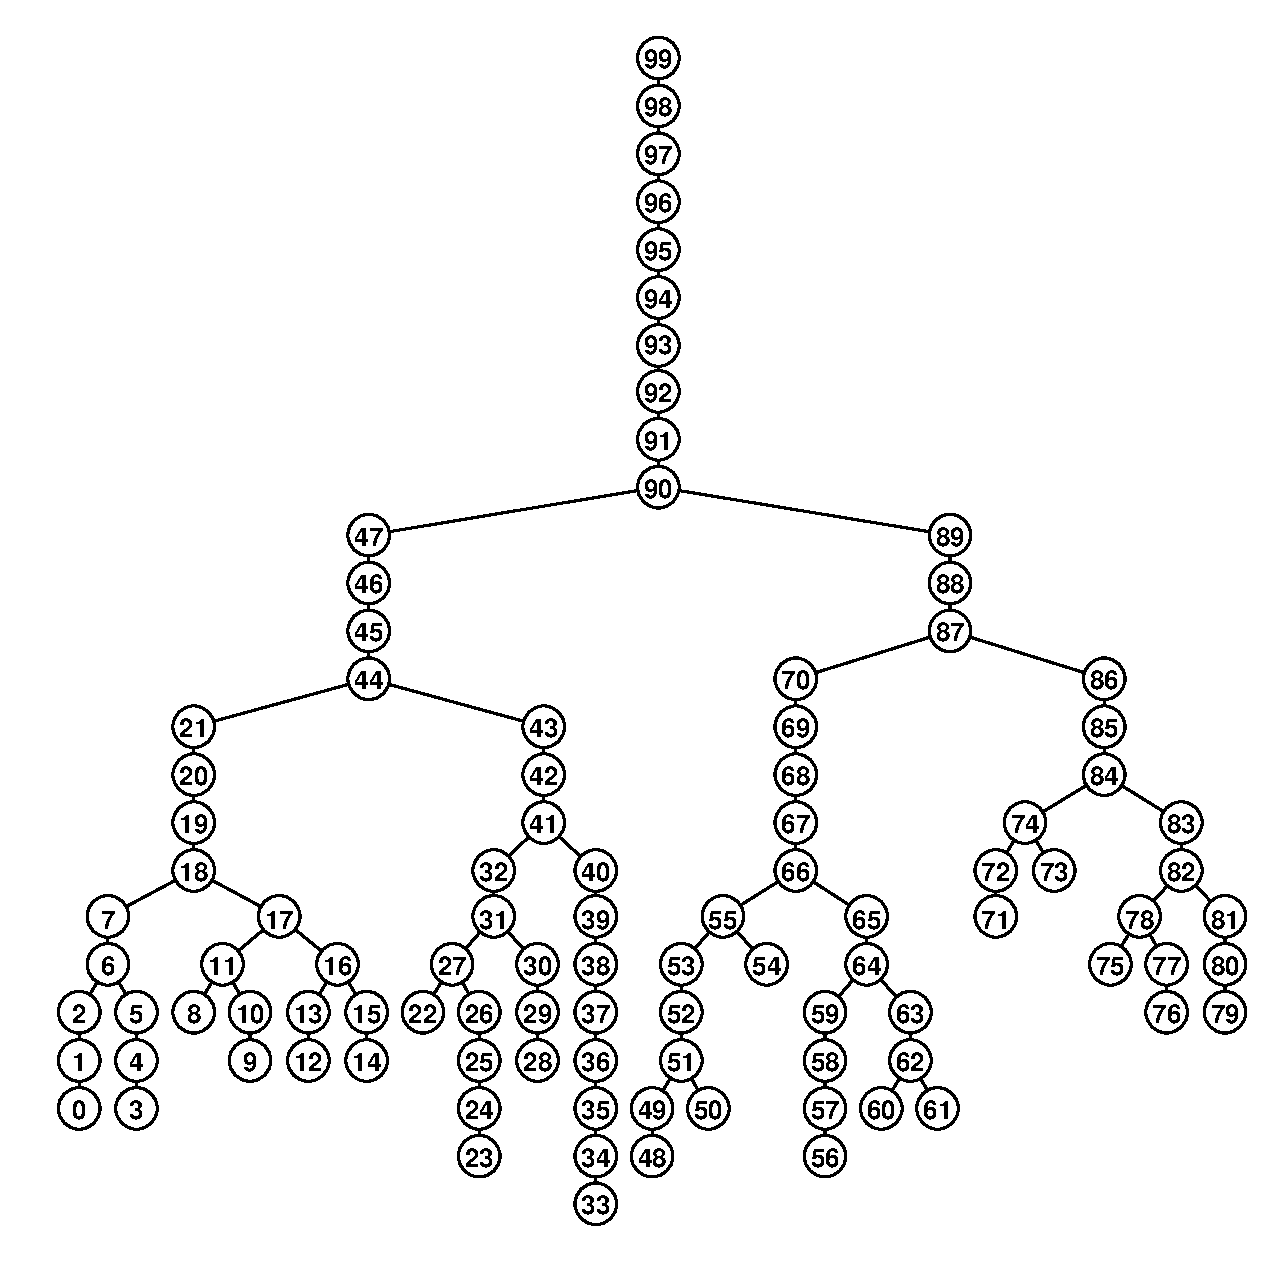
\psfig{file=R2D100vtx.eps,width=5.0in,height=5.00in}
}
\end{center}
\end{figure}
\par
The elimination tree illustrates the dependence of the vertices.
The basic  rule is that a vertex {\it depends} only on its descendents
and will {\it affect} only its ancestors.
It should be clear that the tree allows us to identify independent,
parallel computation.
For example, the computation of the factor entries in the 
subtree rooted at vertex 47 is completely independent of the
subtree rooted at vertex 89, so we could identify one process to
compute the left subtree and another to compute the right subtree.
\par
While the vertex elimination tree is useful to communicate the data
dependencies, it is not a good granularity on which to
base a factorization or solve, in serial or in parallel.
It is important to group vertices together in some meaningful way
to create larger data structures that will be more efficient with
respect to storage and computation.
The first step in this direction is to group together vertices
that form a chain with no branches in the tree.
Using this grouping we generate the {\it fundamental supernode tree}
given in the bottom of Figure~\ref{fig:R2D100-tree-front}.
\begin{figure}[htbp]
\caption{Top: vertex elimination tree with the vertices mapped to
the fundamental supernode that contains them. 
Bottom: fundamental supernode tree.}
\label{fig:R2D100-tree-front}
\begin{center}
\mbox{
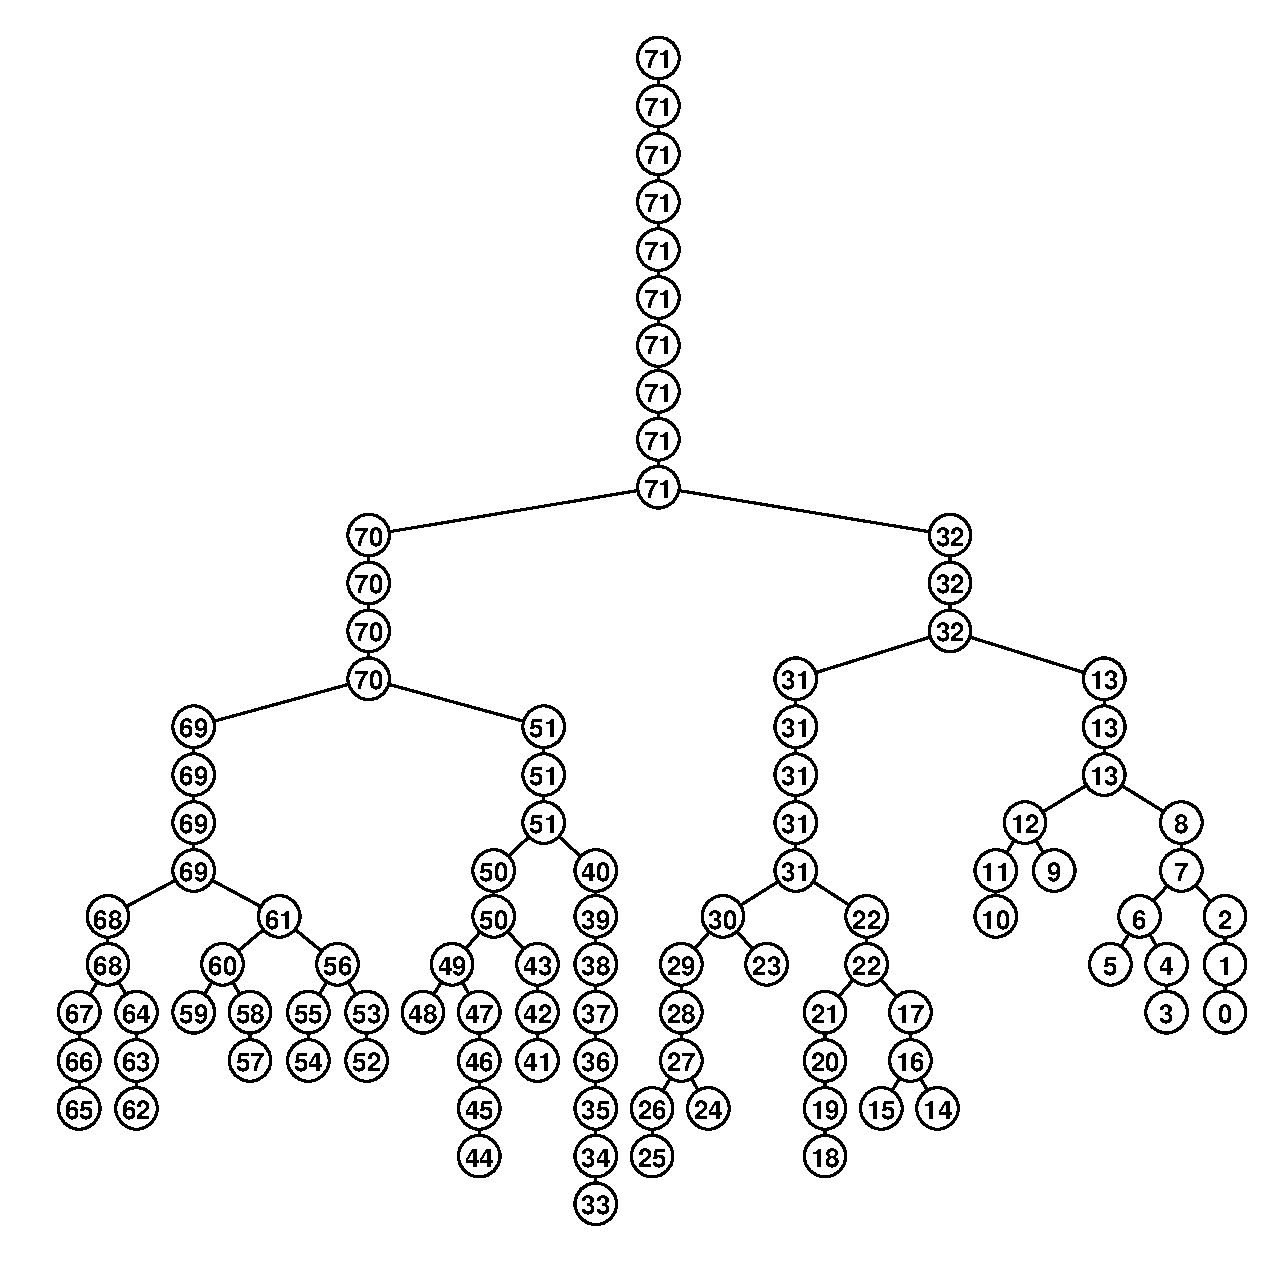
\psfig{file=R2D100vtxmap.eps,width=5.0in,height=5.00in}
}
\par
\mbox{
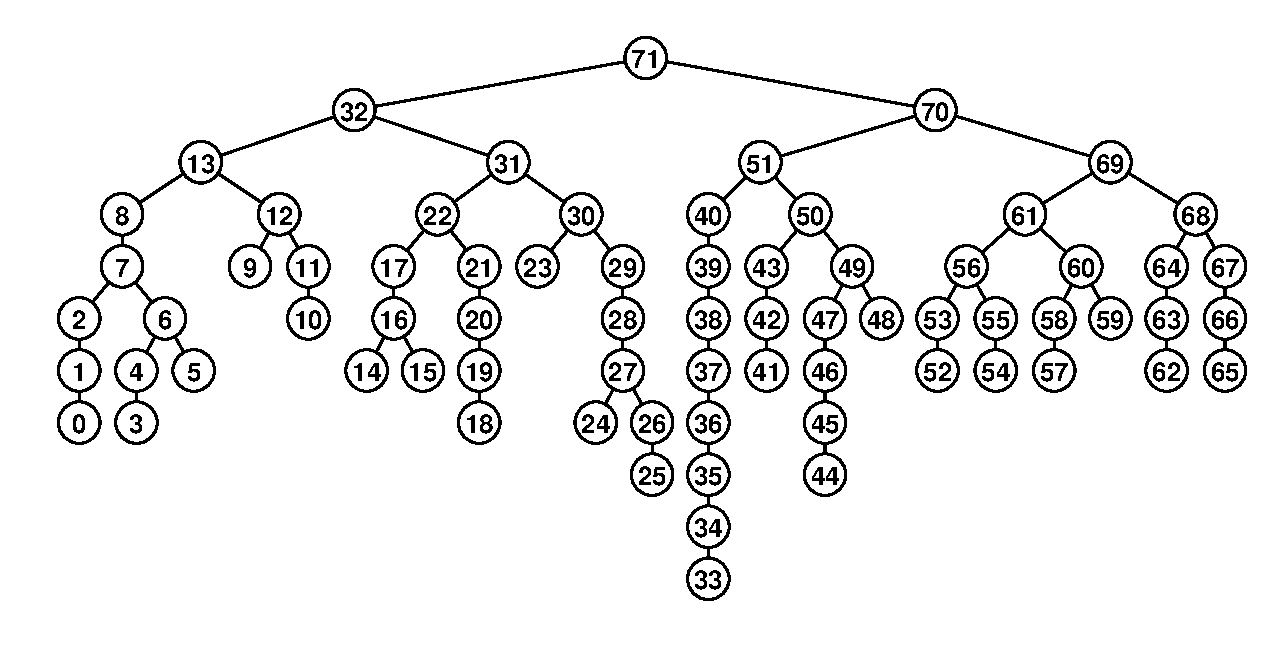
\psfig{file=R2D100front.eps,width=5.0in,height=2.50in}
}
\end{center}
\end{figure}
\par
A factorization based on the fundamental supernode tree requires
no more operations than one based on the vertex elimination tree.
There are many small supernodes at the lower levels of the tree. 
By {\it amalgamating} small but connected sets of supernodes together into larger
supernodes we can reduce the overhead of the processing all of the small
supernodes at the expense of adding
entries to the factors and operations to compute the factorization.
This amalgamation of supernodes generally leads to an overall increase in 
efficiency.  We call the result of the {\it amalgamated} supernode tree.
\par
The tree in the bottom of Figure~\ref{fig:R2D100-tree-comp} was
obtained by allowing up to twenty logically zero entries into the
block column for a supernode.
The top tree shows the fundamental supernodes mapped to their
amalgamated supernodes.
\par
\begin{figure}[htbp]
\caption{Top: fundamental supernode tree with the supernodes mapped to
the amalgamated supernode that contains them. 
Bottom: amalgamated supernode tree.}
\label{fig:R2D100-tree-comp}
\begin{center}
\mbox{
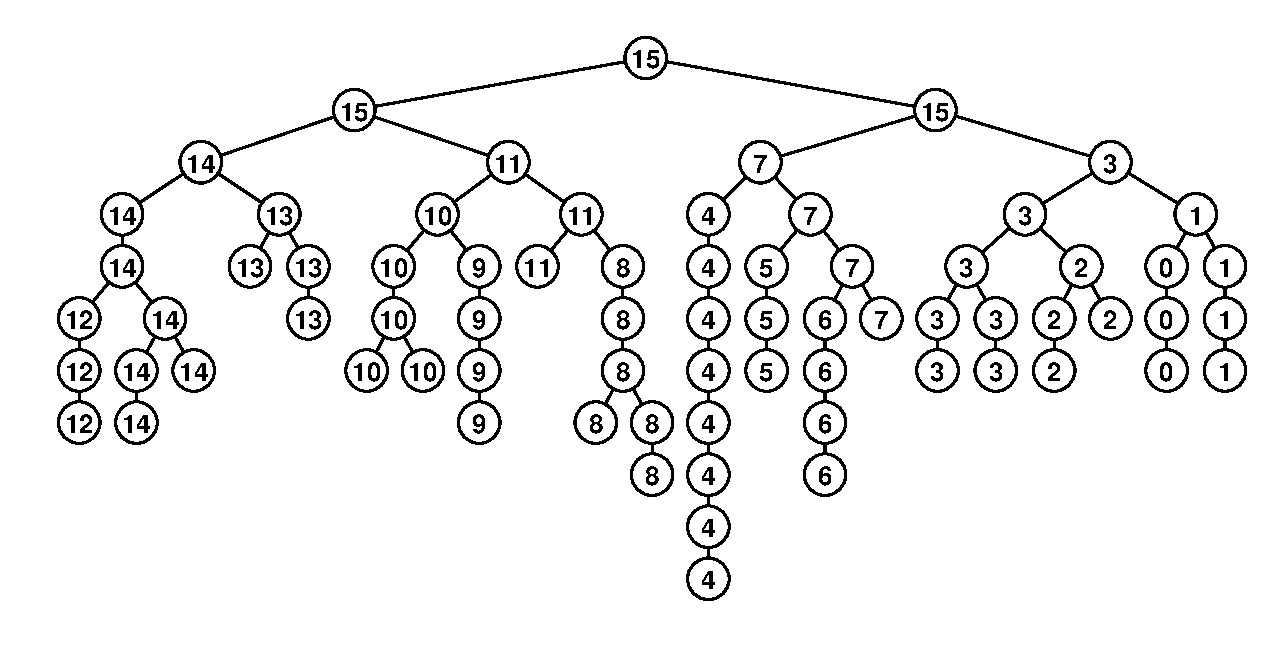
\psfig{file=R2D100frontmap.eps,width=5.0in,height=2.50in}
}
\par
\mbox{
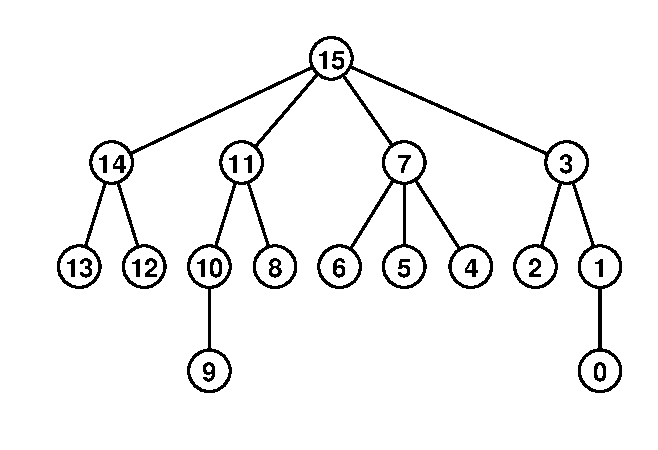
\psfig{file=R2D100comp.eps,width=3.0in,height=2.00in}
}
\end{center}
\end{figure}
\par
There is one final step to constructing the tree that governs the
factorization and solve.
Large matrices will generate large supernodes at the topmost levels
of the tree.
For example, a $k \times k \times k$ grid with a 27 point finite
difference operator, when ordered by nested dissection, has a root
supernode with $k^2$ rows and columns.
The data structure for a top level supernode can be very large,
too large to fit into memory.
In a parallel environment, we follow the convention that each node
in the tree is handled by one process.
Having a very large node at the top levels of the tree will
severely decrease the parallelism available to the computations.
\par
The solution to both problems, large data structures and limited
parallelism, is to split large supernodes into pieces.
We can specify a maximum size for the nodes in the tree, and split
the large supernode into pieces no larger than this maximum size.
This will keep the data structures to a manageable size and increase
the available parallelism.  We call the resulting tree the {\it front}
tree because it represents the final computational unit for the
factorization, the frontal matrix.
\par
The amalgamated supernode tree has been transformed so that except for
the leaf nodes, which are not changed, no node in the tree has more 
than four vertices.
The new tree is given on the left
of Figure~\ref{fig:R2D100-tree-split},
while the right tree shows maps the nodes back to the amalgamated
supernode tree.
Splitting large nodes into smaller nodes will not increase the
factor storage or operation counts.
\par
\begin{figure}[htbp]
\caption{Left: tree after the large supernodes have been split.
Right: tree with nodes mapped back to their amalgamated supernode.}
\label{fig:R2D100-tree-split}
\begin{center}
\mbox{
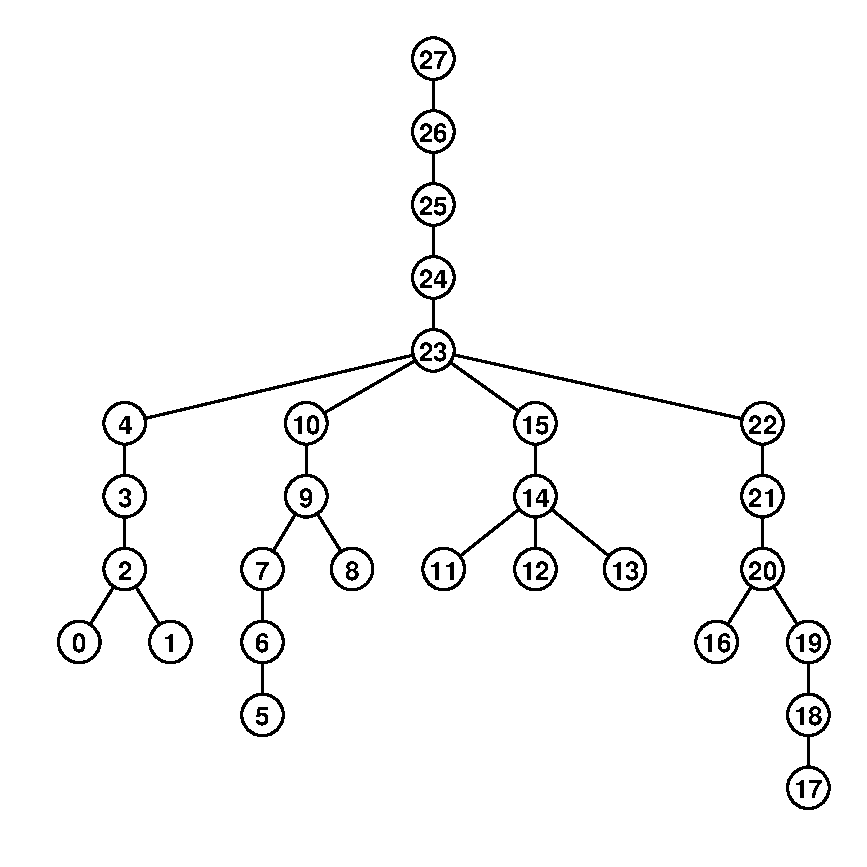
\psfig{file=R2D100split.eps,width=3.00in,height=3.000in}
}
\quad
\mbox{
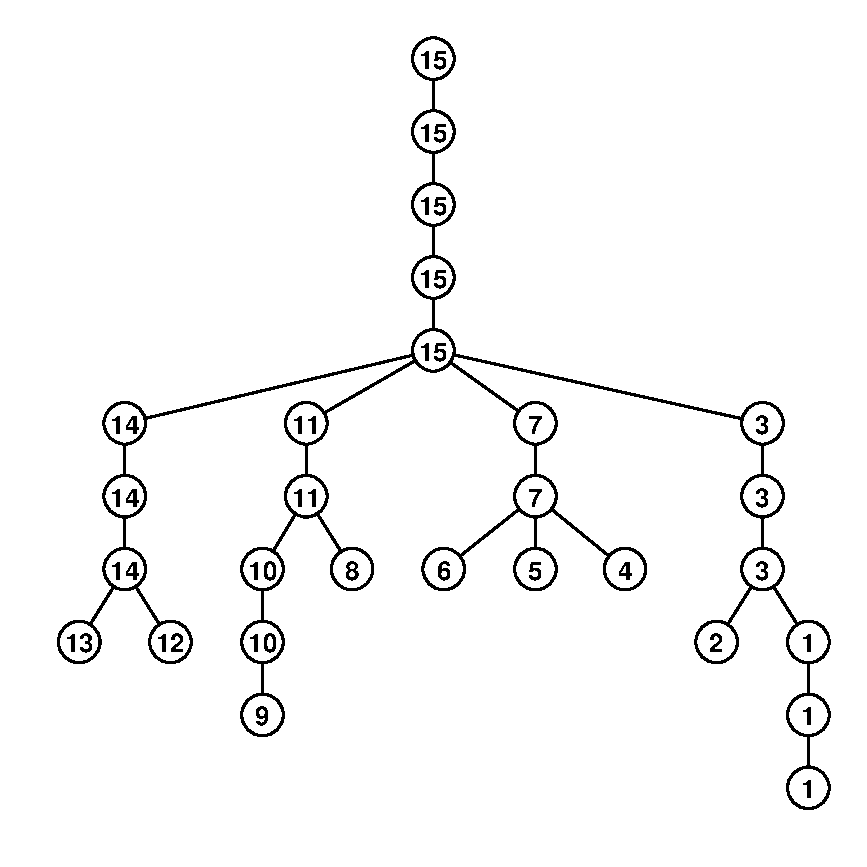
\psfig{file=R2D100splitmap.eps,width=3.00in,height=3.000in}
}
\end{center}
\end{figure}
\par
This front tree is now the defining
structure for the numerical factorization and solve steps.  The structure
of the front tree defines the order of the computations that will be
carried out in the factorization and the solve.  The methods for
almagamating and splitting to produce the front tree is found in
Section~\ref{chapter:manipulating:ETree}.
\par
\subsection{Matrix factorization and solves}
\label{subsection:intro:solve}
\par
One of the most important design consideration for our numeric
software is to support pivoting for numerical stability.
Much of the time pivoting for stability is not needed --- 
when matrices are diagonally dominant or well conditioned positive definite --- 
but there are
cases where pivoting is crucial.
\par
For symmetric matrices we use the fast Bunch-Parlett algorithm
to choose $1 \times 1$ or $2 \times 2$ pivots
\cite{ash95-AGL}.
For non-symmetric matrices we use its analogue.
It has recently come to our attention that this
pivoting strategy has been known as {\it rook pivoting}
\cite{fo96-rook}, \cite{ne92-rook}.
We compute the factorization
$P L D U Q$ or $P U^T D U P^T$
where $L$ is unit lower triangular,
$U$ is unit upper triangular,
and $P$ and $Q$ are permutation matrices.
When pivoting is enabled, the magnitude of entries in $L$ and
$U$ are bound by some user supplied tolerance.
\par
For the {\bf SPOOLES} library we chose to implement the fan-in 
algorithm for the numerical factorization
\cite{ash90-fan-in}.  When it is time
to begin the computations for a given front, the processor owning
the rows and columns for that front receive the modification to 
that front from previously computed fronts which are owned by other
processors.  The incoming modification is computed by the processor
that owns the previously computed front.
